\section{Isomer Branching Ratio}

With our dual ablation system, we can reliably co-trap carbon and beryllium ions and introduce cold molecules from the CBGB. Introducing water entrained in a cold neon buffer gas beam, we can see the reaction products due to these collisions. Expected temperature of the buffer gas is 20K, which is defined by the temperature of the inner cell.

We do not expect any reactions to occur with the cold neon buffer gas. We have experimentally verified the absence of new mass peaks when introducing neon into the system with carbon and beryllium ions, only an overall loss rate attributed to elastic collisions within the trap.

Conversely, the water molecules will react readily with both beryllium and carbon ions:

\begin{align}
	C^+ +H_2O & \rightarrow HCO^+ + H \label{r: HCO} \\
	& \rightarrow COH^+ + H \label{r: COH} \\
	Be^+ + H_2O & \rightarrow BeOH^+ + H  \label{r: beoh}
\end{align}

We want to probe the branching ratio of the formyl isomers formed in reactions \ref{r: HCO} and \ref{r: COH} at low temperatures. At room temperatures, the branching ratio has been found to be approximately 84:16 (HCO:COH)\cite{Freeman1987}, but unexplored at lower regimes. We have found that the total reaction rate of \ref{r: HCO}+\ref{r: COH} is approximately 2-3 times larger than that of \ref{r: beoh}, all reaction constants being around Langevin ($10^{-9}$ cm$^3$/s).

To be able to find the branching ratio of the isomer products from reactions \ref{r: HCO} and \ref{r: COH}, we need to be able to separate their masses. 

Unfortunately, there are secondary reactions that also occur on the same time-scale, namely the reaction products from the initial reactions reacting with water again, which also happens around Langevin.

\begin{align}
	HCO^+/COH^+ + H_2O &\rightarrow H_3O^+ + OH \label{r: c2}
\end{align}

\begin{table}[H]
\centering
\label{t: affinities}
\begin{tabular}{ll}
    & Affinity (kcal/mol) \\
CO* & 427               \\
Kr  & 425               \\
HF  & 490               \\
N2  & 495               \\
Xe  & 496               \\
NO  & 531               \\
CO2 & 548               \\
CH4 & 552               \\
HCl & 564               \\
HBr & 569               \\
N2O & 571              \\
*CO & 594
\end{tabular}
\caption{Proton affinities of gasses between formyl isomers where (*) indicates H bonding location.} \label{tab: affinity}
\end{table}

This poses a problem as we need to react away one of the isomers faster than they both become H$_3$O$^+$. Due to the fact that the hydrogen bond is on different molecules, each isomer has a different proton affinity as seen in table \ref{t: affinities} \cite{Love1987TheAffinity}

\subsection{$^{15}$N$_2$ Titration}

\subsection{CO$_2$ Titration}

From table \ref{tab: affinity}, we see that CO$_2$ is an option to titrate the reaction products. From literature, we find that this should not interfere with the determination of the products of interest.

\begin{align}
	\text{Be}^+ + \text{CO}_2 & \rightarrow \text{no reaction} \\
	\text{C}^+ + 
\end{align}

\section{Be$^+$ + O$_2$}

Beryllium metal is ablated with an Nd:YAG laser and trapped in a linear Paul trap. Laser cooling is applied with a 313nm laser. Pure O$_2$ gas is introduced into the chamber via leak valve to react with the ions. Remaining reactants and charged reaction products are ejected into a time-of-flight mass spectrometer (TOF) where the various masses of ions can be determined.

When the Be$^+$ is excited from the $^2$S$_{1/2}$ to the $^2$P$_{3/2}$ manifold, we find the energetically allowed channels to be:

\begin{align}
    \text{Be}^+(^2\text{P}_{3/2}) + \text{O}_2 & \to \text{O}_2^+ + \text{Be} \label{eq: o2+} \\
    & \to \text{BeO}^+ + \text{O}_2 \label{eq: beo+} \\
    \text{Be}^+(^2\text{P}_{3/2}) + \text{H$_2$O} & \to \text{BeOH}^+ + \text{H} \\
    \text{Be}^+(^2\text{P}_{3/2}) + \text{H}_2 & \to \text{BeH}^+ + \text{H} \\
    \text{BeH}^+ + \text{H$_2$O} & \to \text{BeOH}^+ + \text{OH}
\end{align}

Without excitation into the $^2$P$_{3/2}$ manifold, reactions \ref{eq: o2+} and \ref{eq: beo+} are endothermic by 2.75eV and 1.1eV, respectively. 

Despite the fact that reaction \ref{eq: beo+} is energetically allowed, it is never seen with laser cooling.

Without 313nm light, the Be$^+$ ions stay in the $^2$S$_{1/2}$ ground state, but with a ion trap depth > 4eV, there are portions of the ion cloud with enough energy to still proceed with the production of BeO$^+$. Without the laser cooling, we observe the disappearance of BeO$^+$ from the trap due to exciting the molecule into a pre-dissociative state.

\begin{figure}[H]
\centering
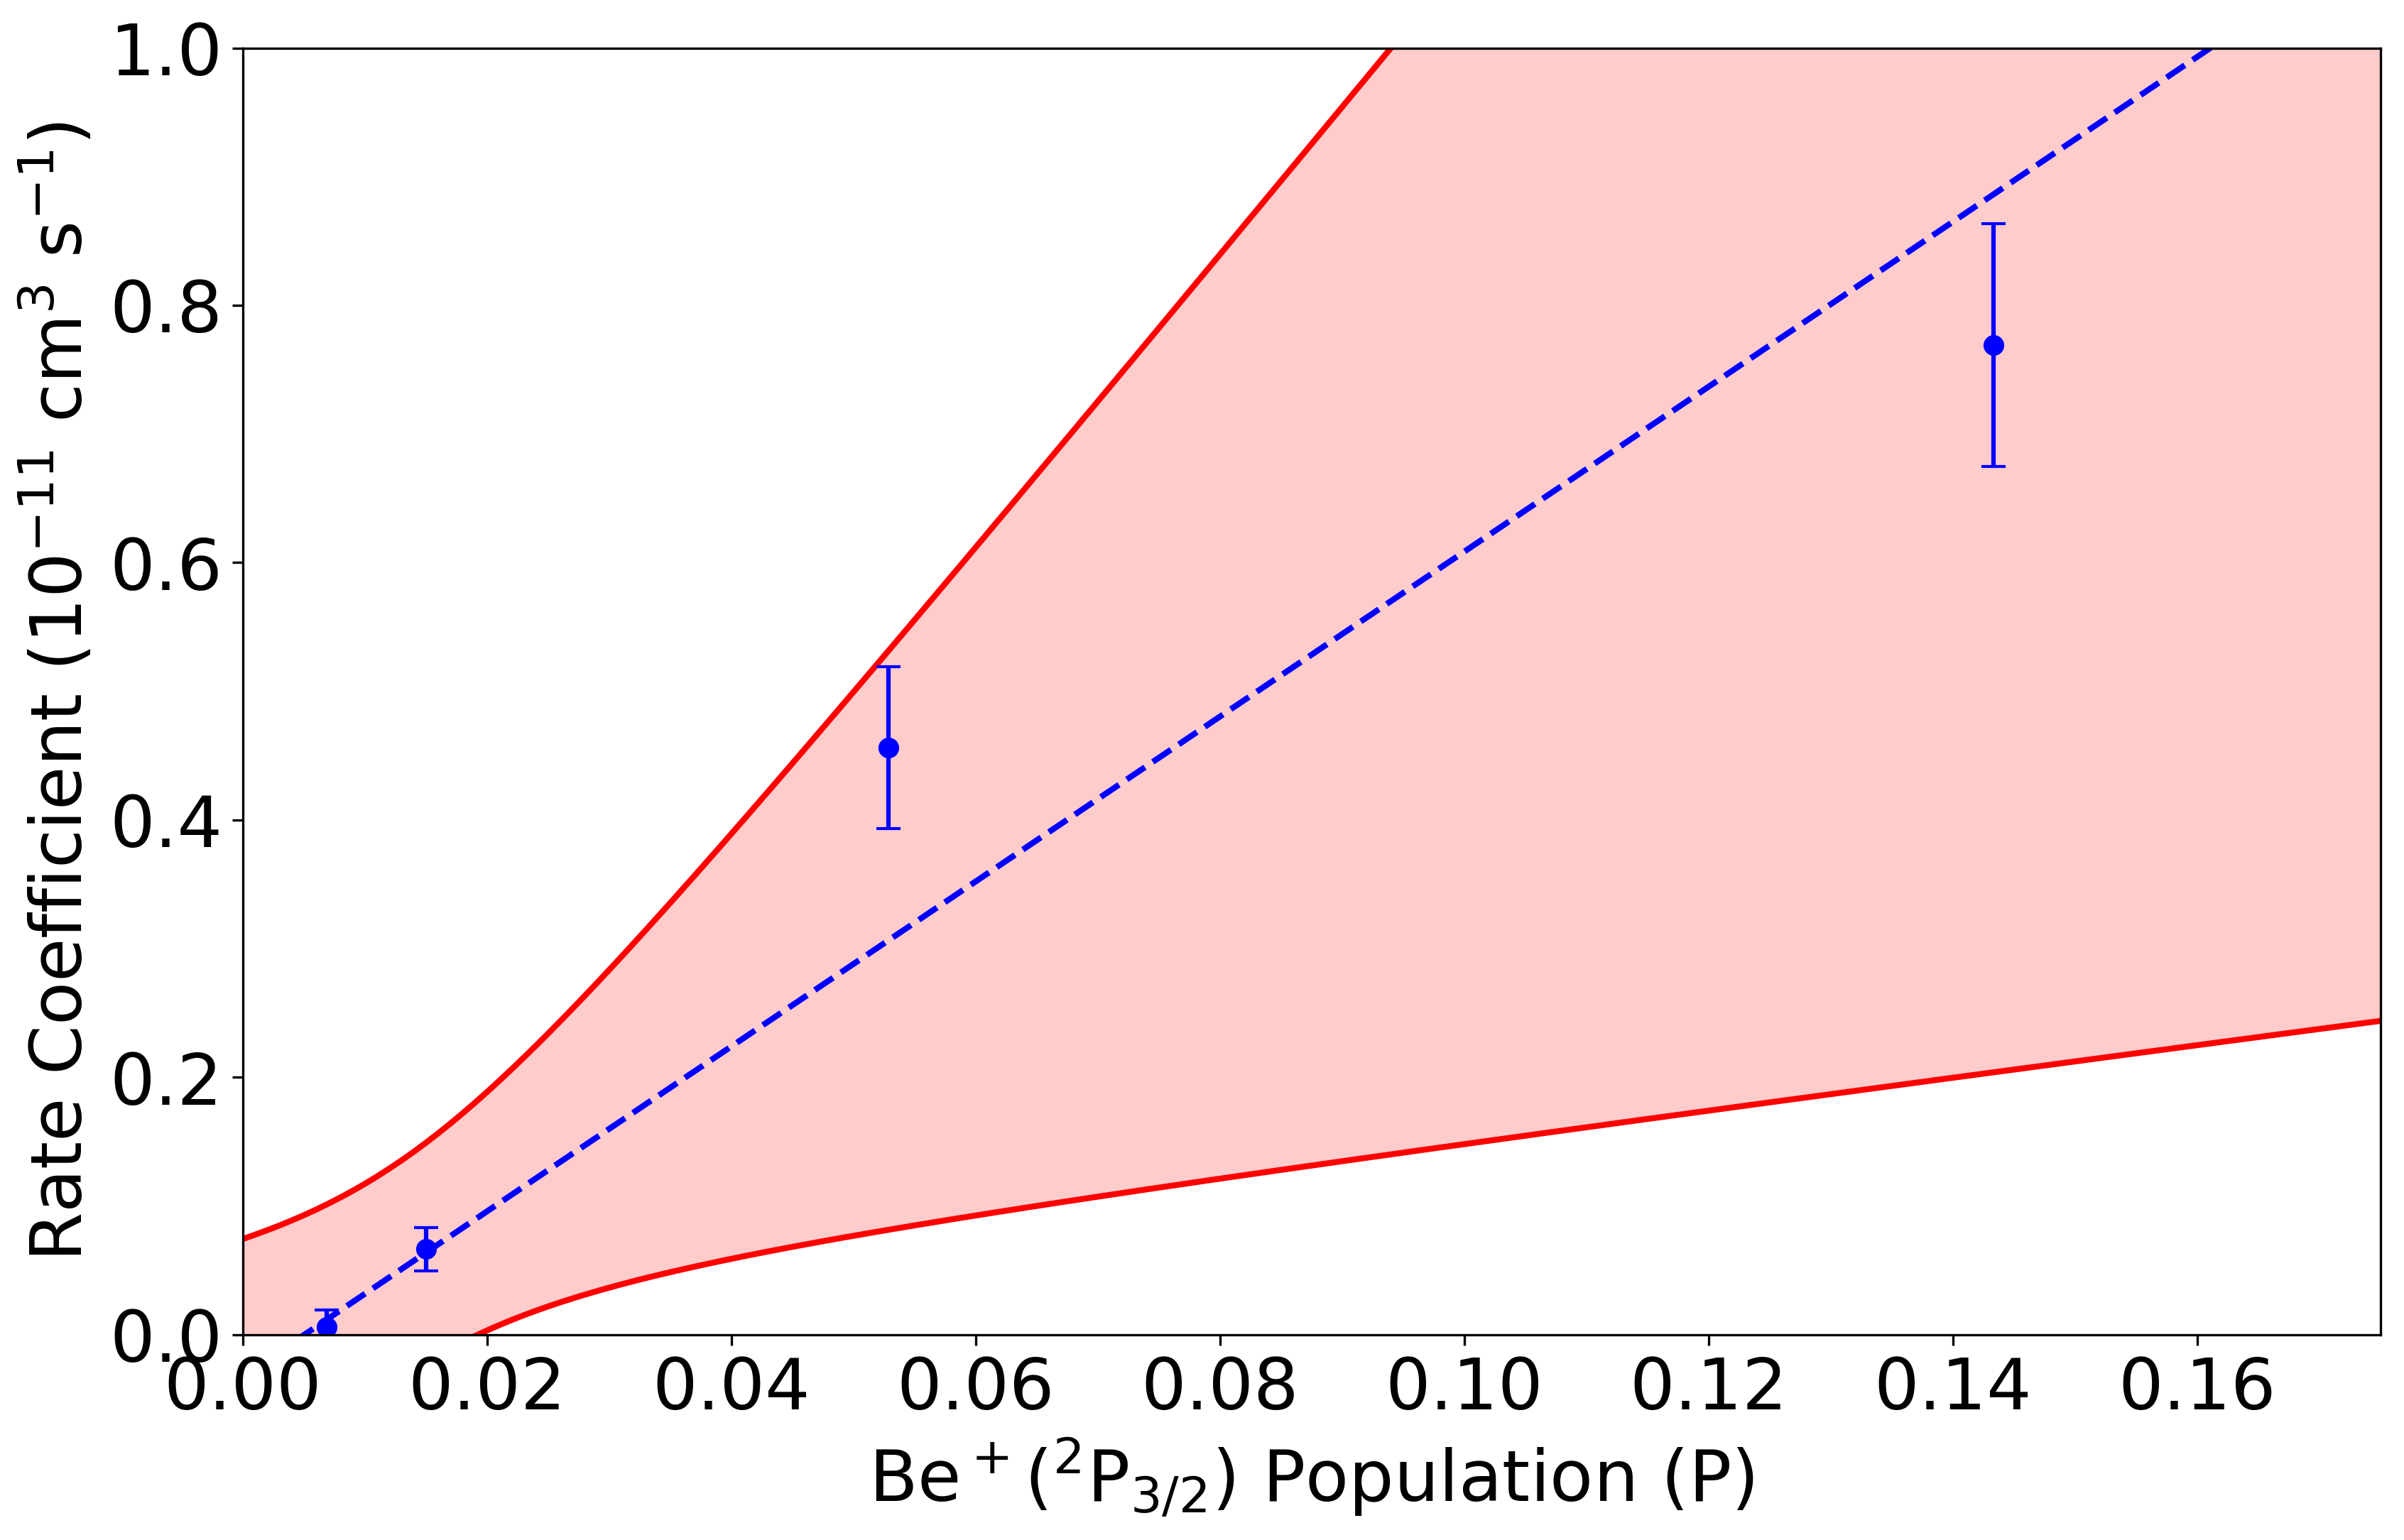
\includegraphics[width=0.7\textwidth]{images/beo_p_state.png}
\caption{\label{fig: p-state} A linear dependence on the rate constant for reaction \ref{eq: o2+} as a function of P state excitation. $k = (6 \pm 1) \times 10^{-11} P + (-0.03 \pm 0.16) \times 10^{-11}$}
\end{figure}

% \begin{figure}[H]
% \centering
% \includegraphics[width=0.5\textwidth]{p_state_no_b.png}
% \caption{\label{fig: p-state} A linear dependence on the rate constant for reaction \ref{eq: o2+} as a function of P state excitation. Fit $(5.45 \pm 1.03) \times 10^{-11} P$}
% \end{figure}

\begin{figure}[H]
\centering
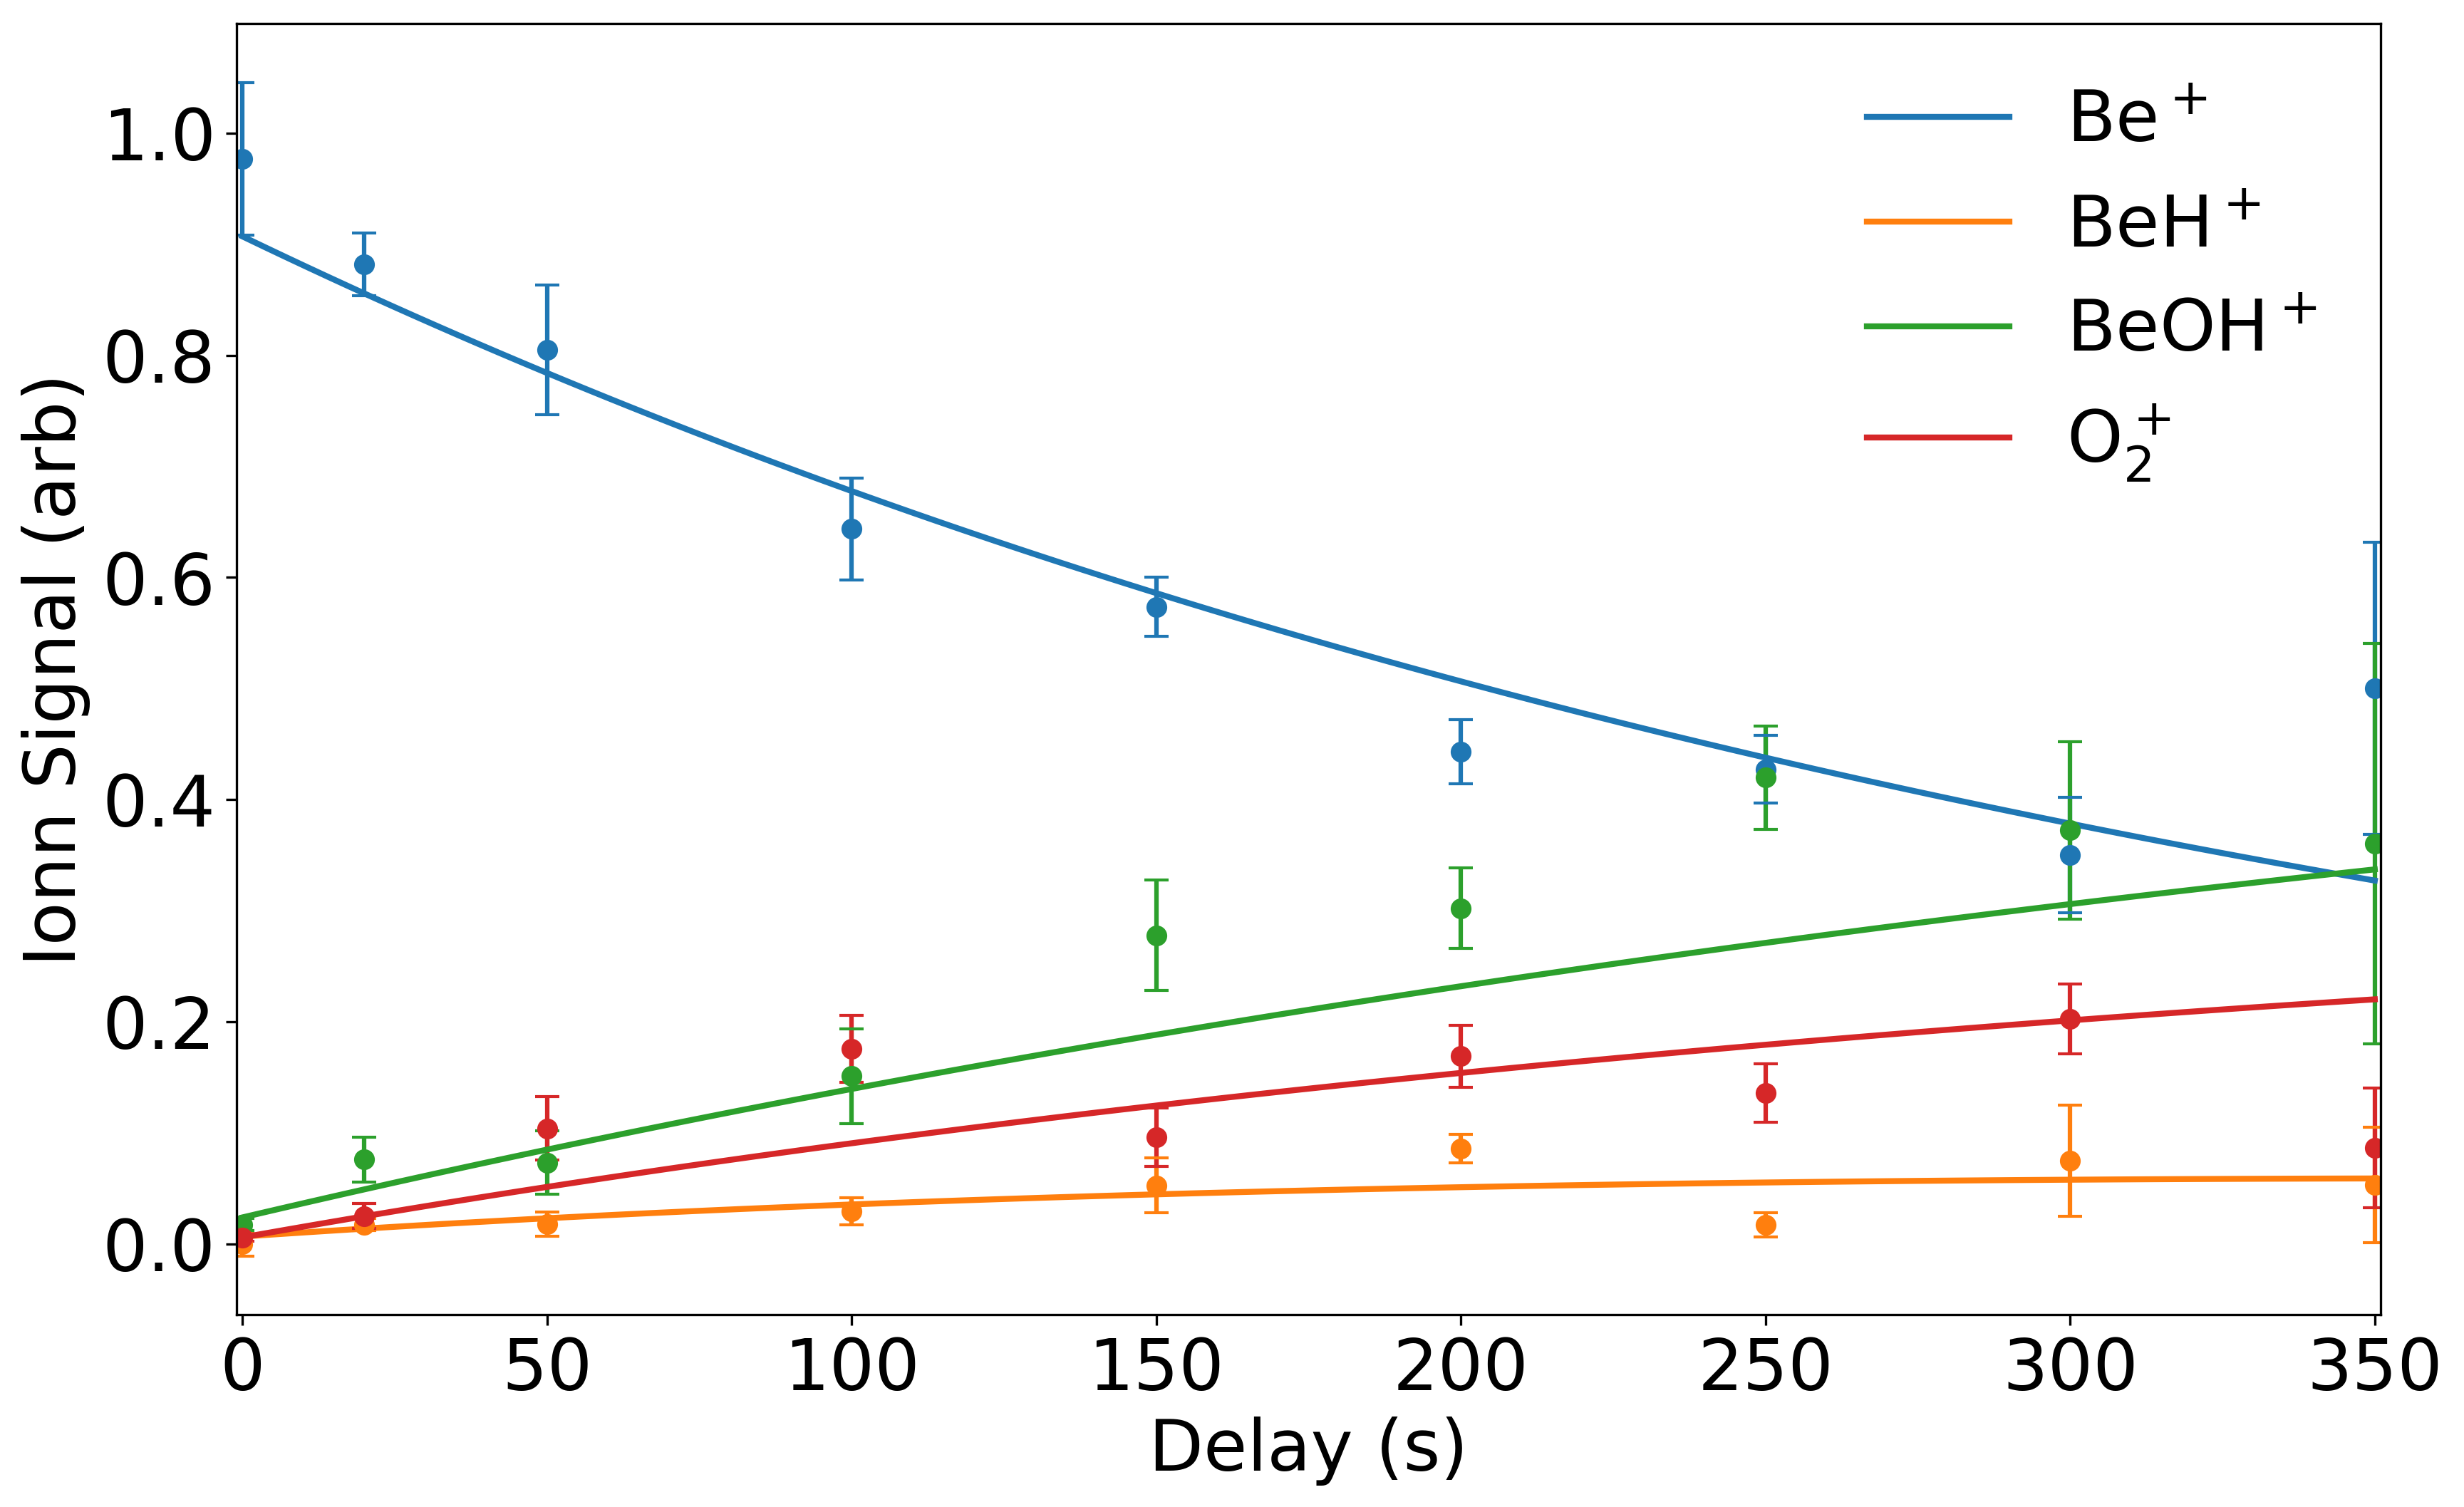
\includegraphics[width=0.7\textwidth]{images/beo_laser_fit.png}
\caption{\label{fig: laser fit} Shared fitting of trapped products with 14\% p-state excitation.}
\end{figure}

\begin{figure}[H]
\centering
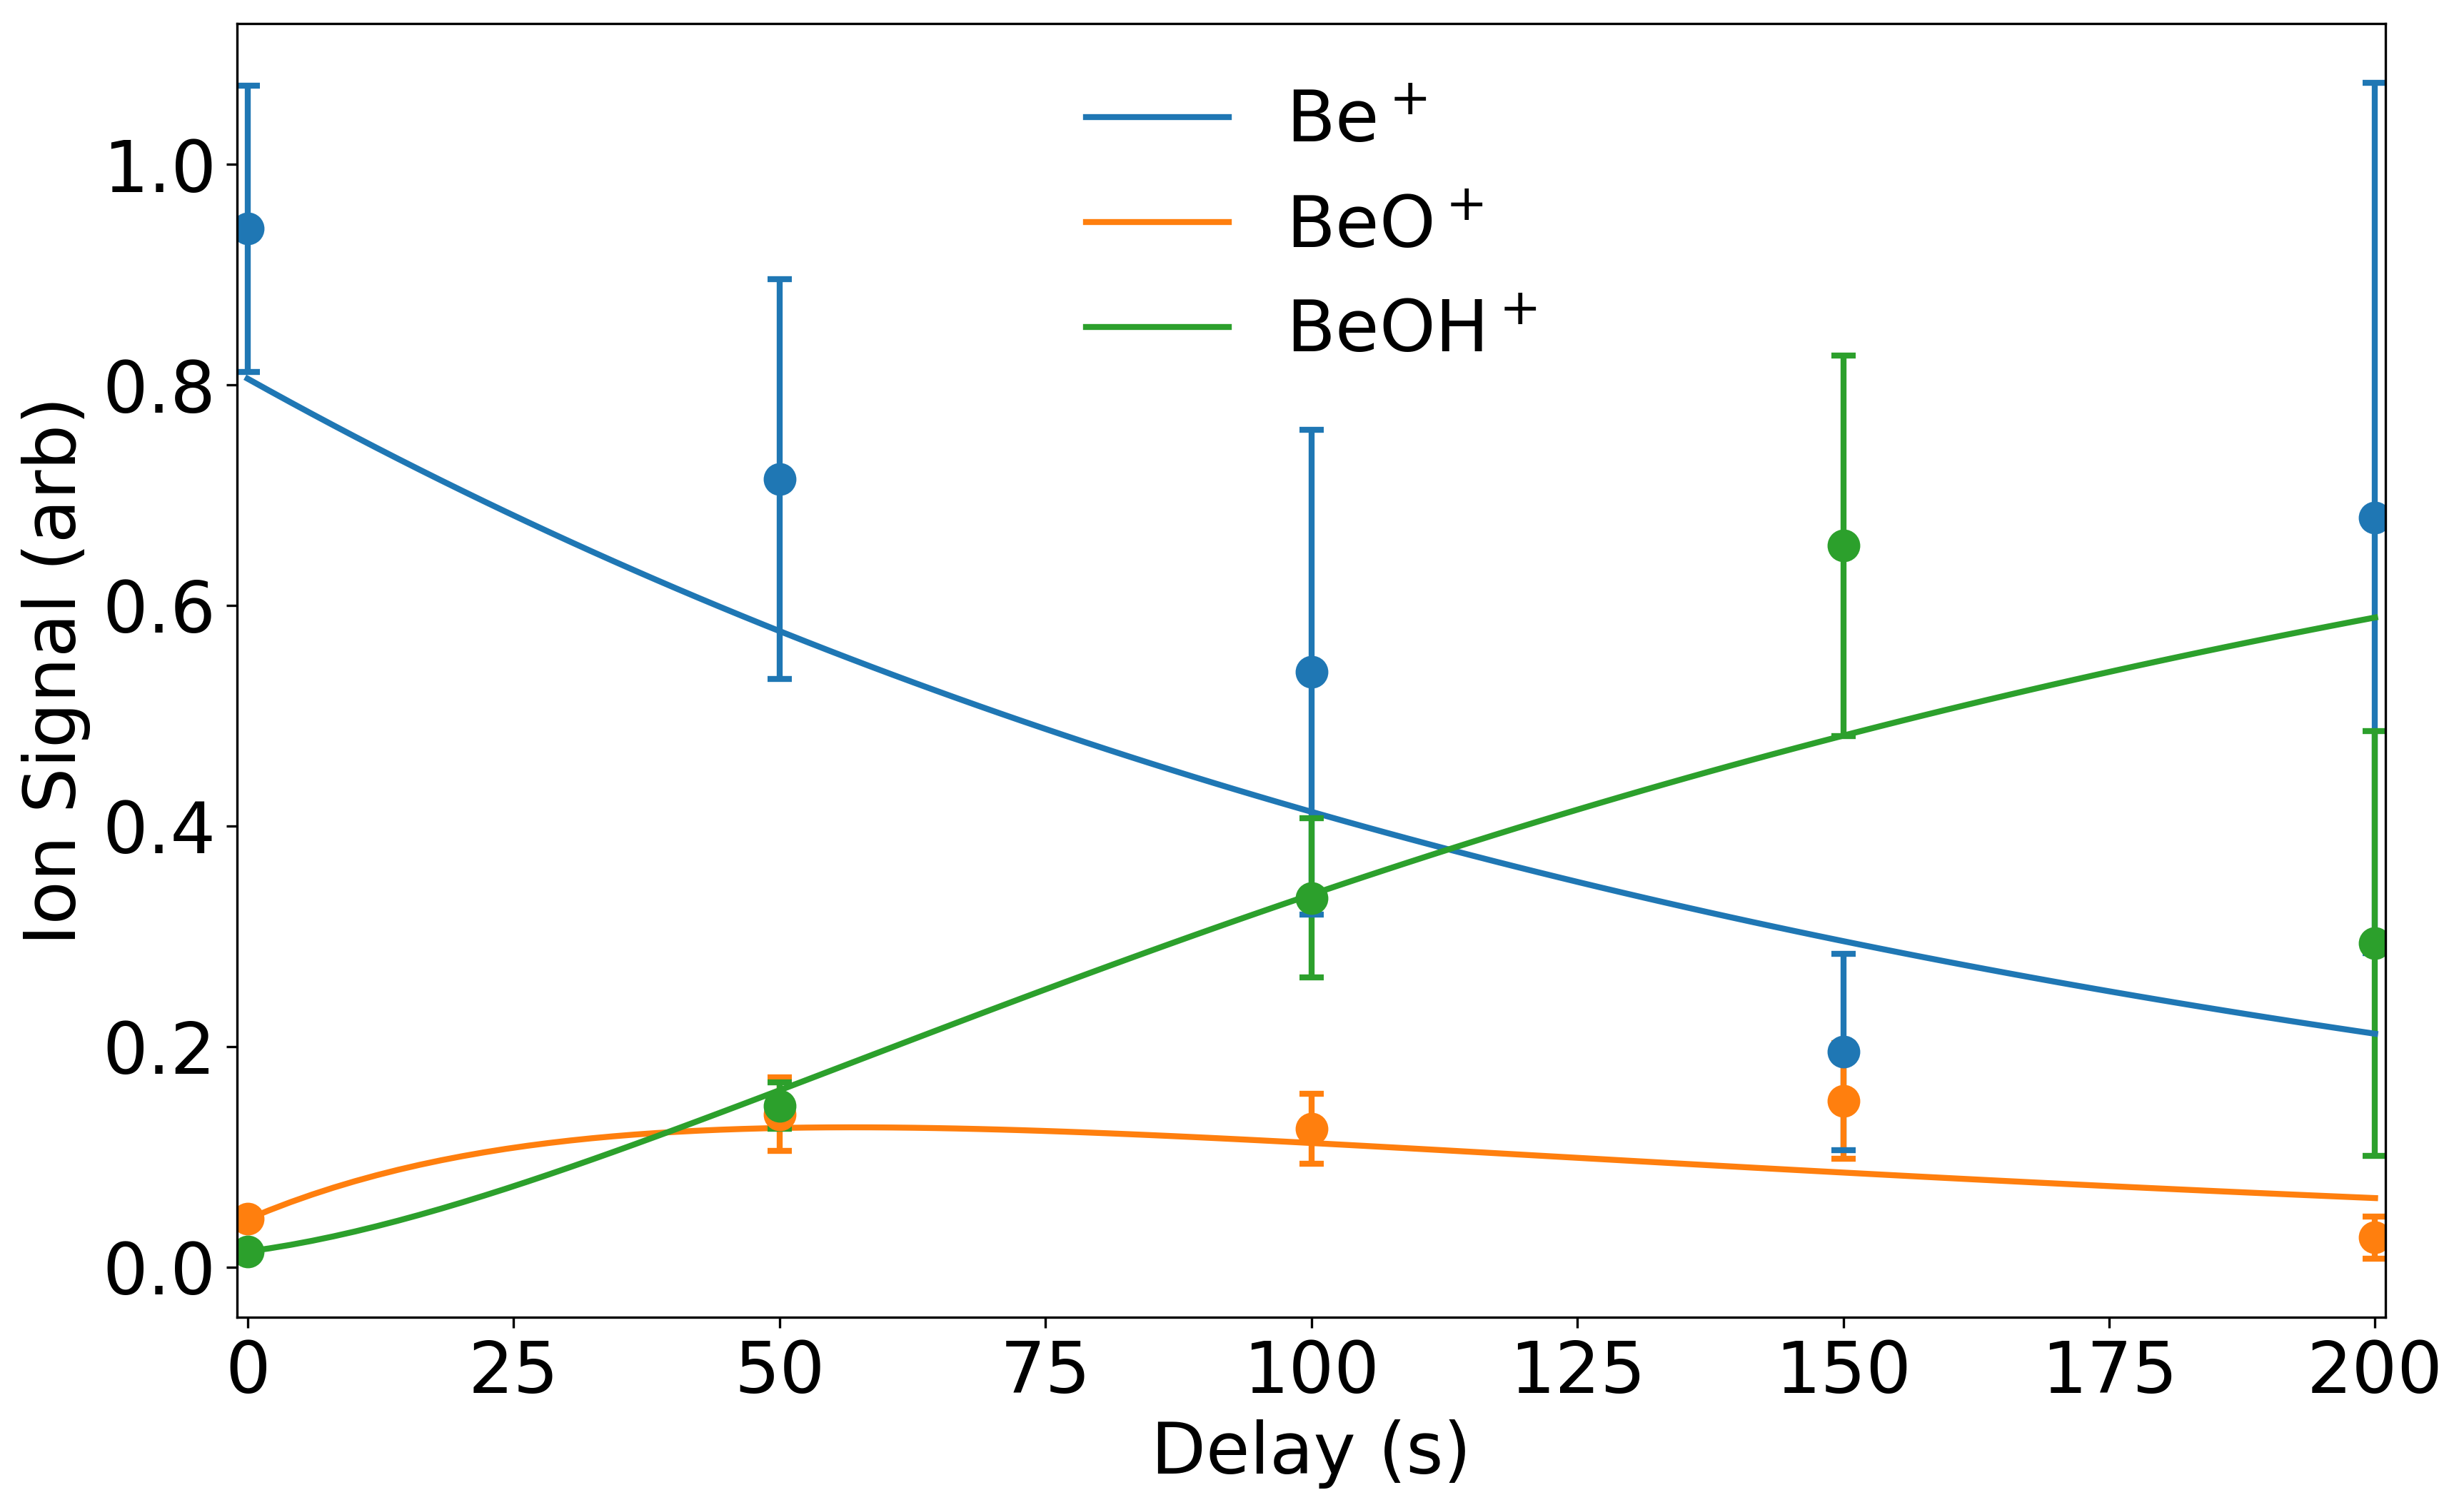
\includegraphics[width=0.7\textwidth]{images/beo_no_laser_fit.png}
\caption{\label{fig: no laser fit} Shared fitting of trapped products with 14\% p-state excitation.}
\end{figure}

\begin{figure}[H]
\centering
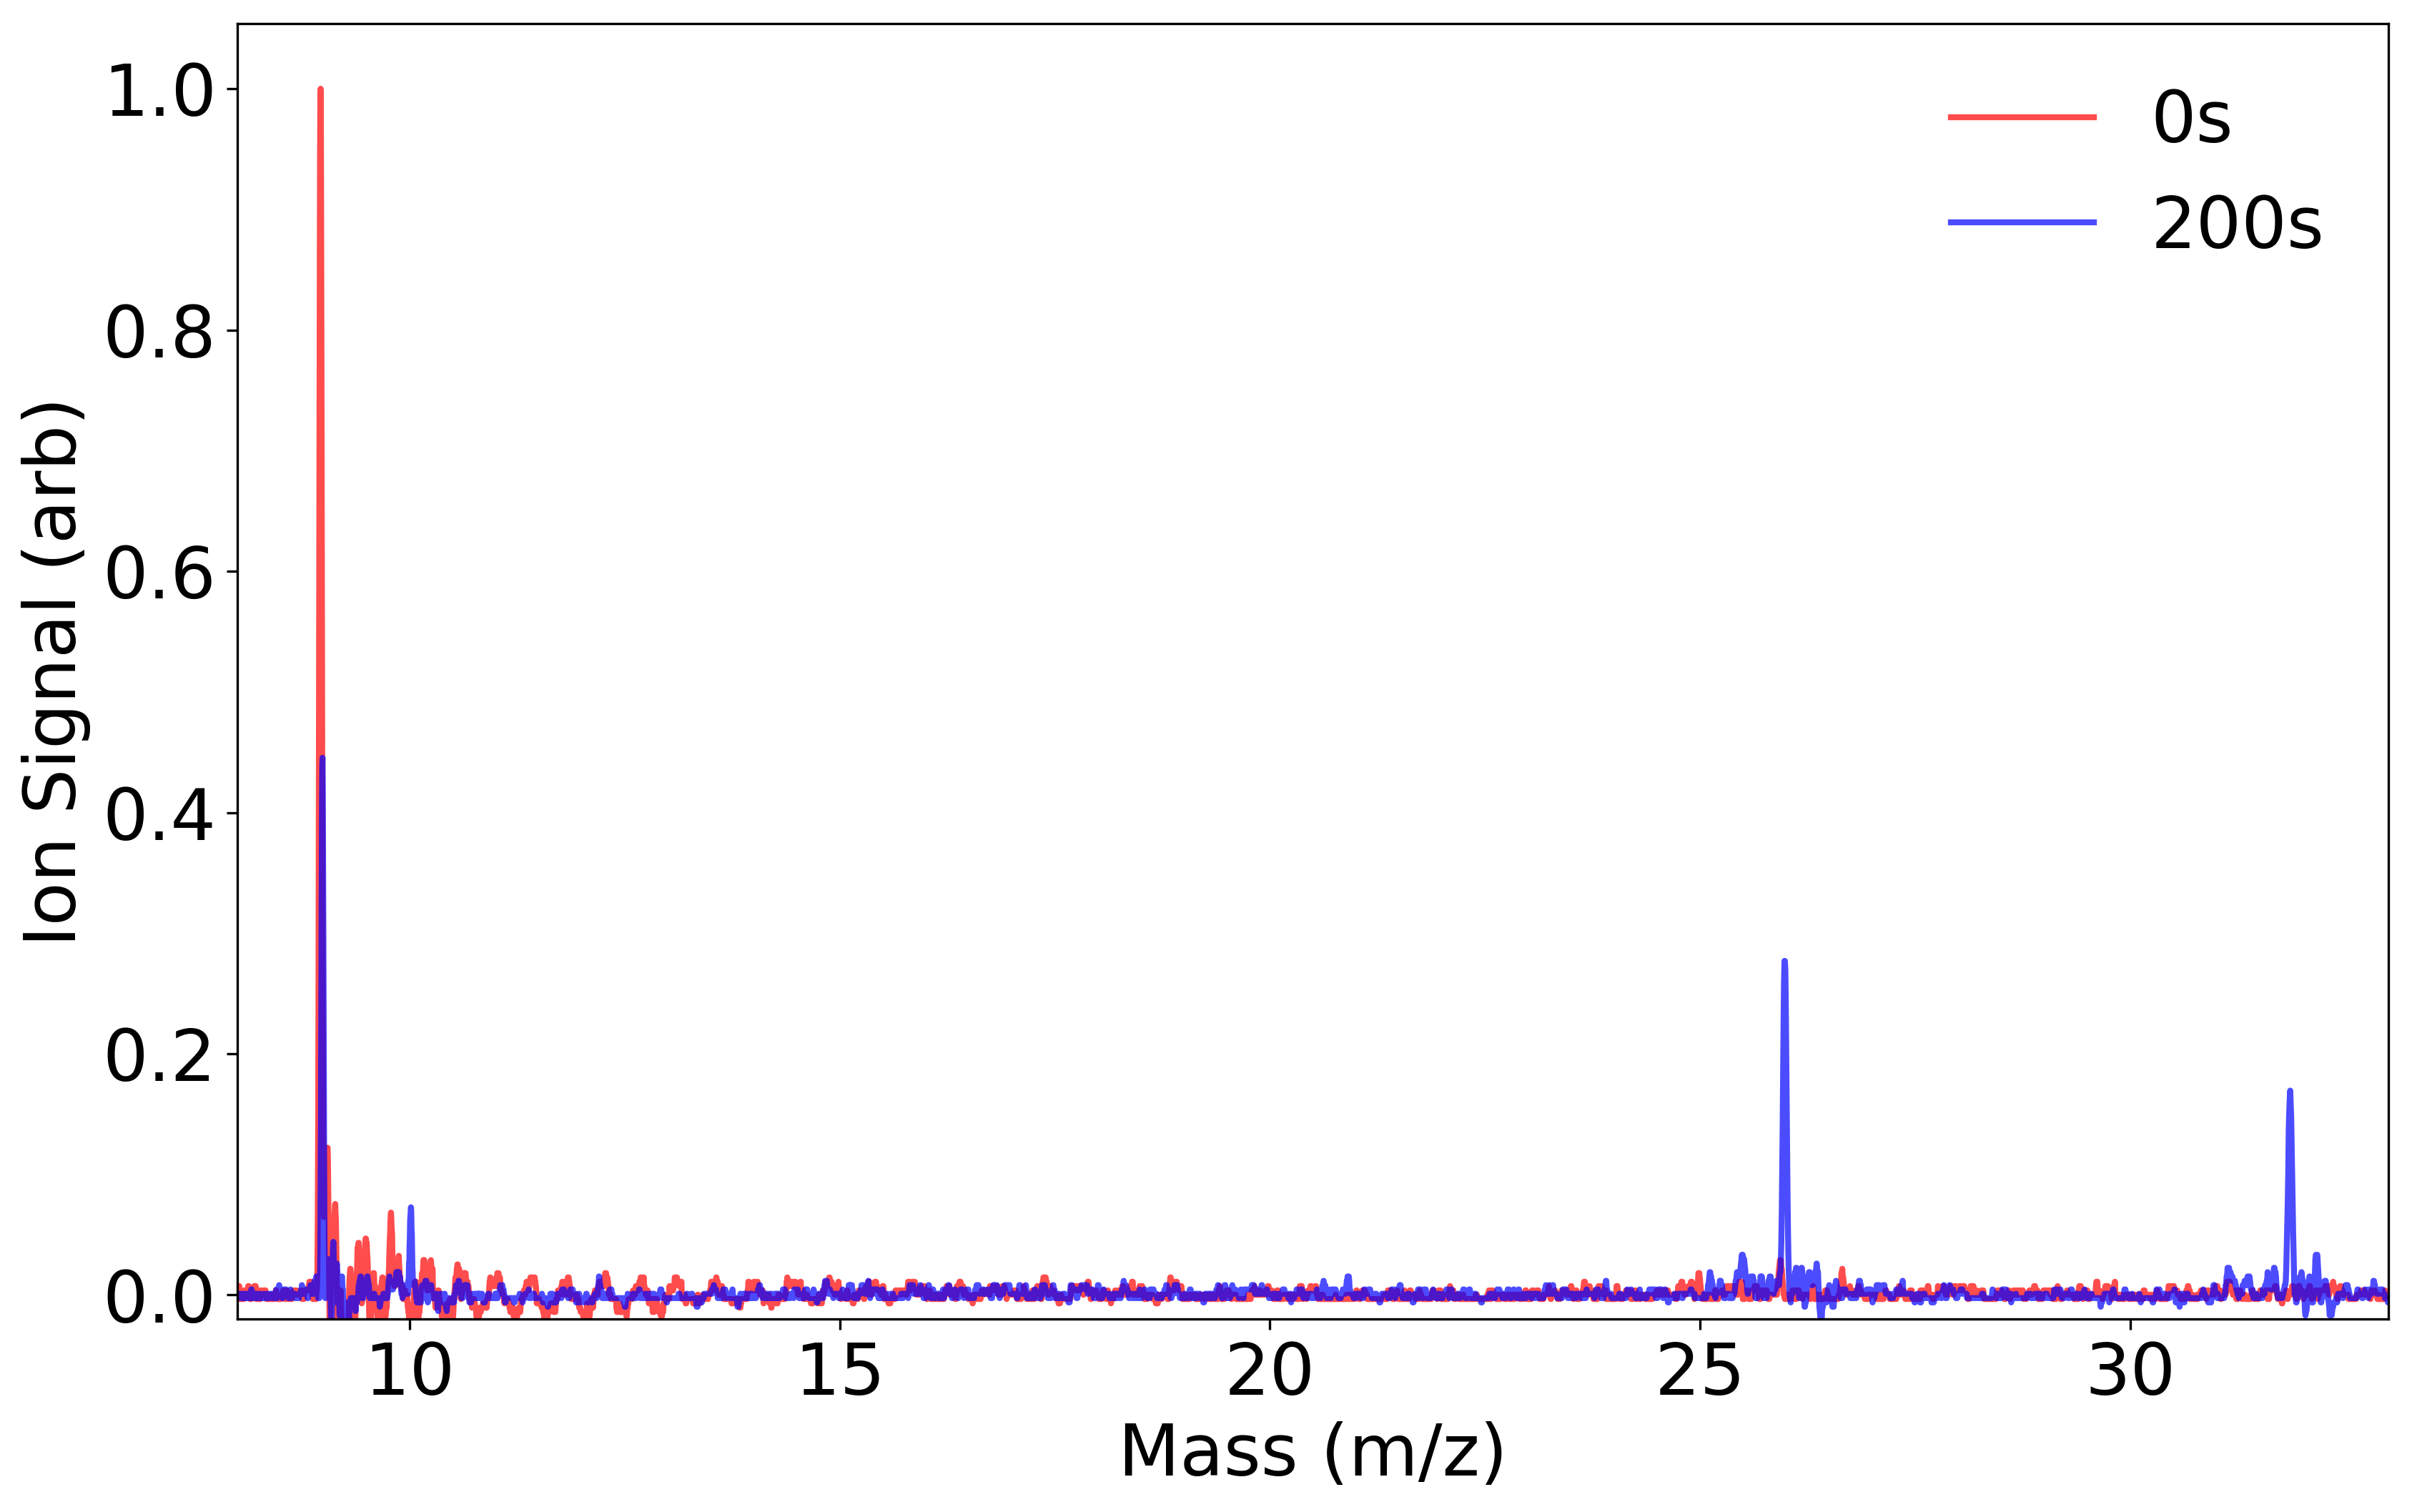
\includegraphics[width=0.7\textwidth]{images/beo_laser_TOF.png}
\caption{\label{fig: laser TOF} TOF traces for data taken with 14\% p-state excitation at 0s and 200s showing no products at 0s, but distinct peaks for reaction products BeH$^+$, BeOH$^+$, and O$_2^+$.}
\end{figure}

\begin{figure}[H]
\centering
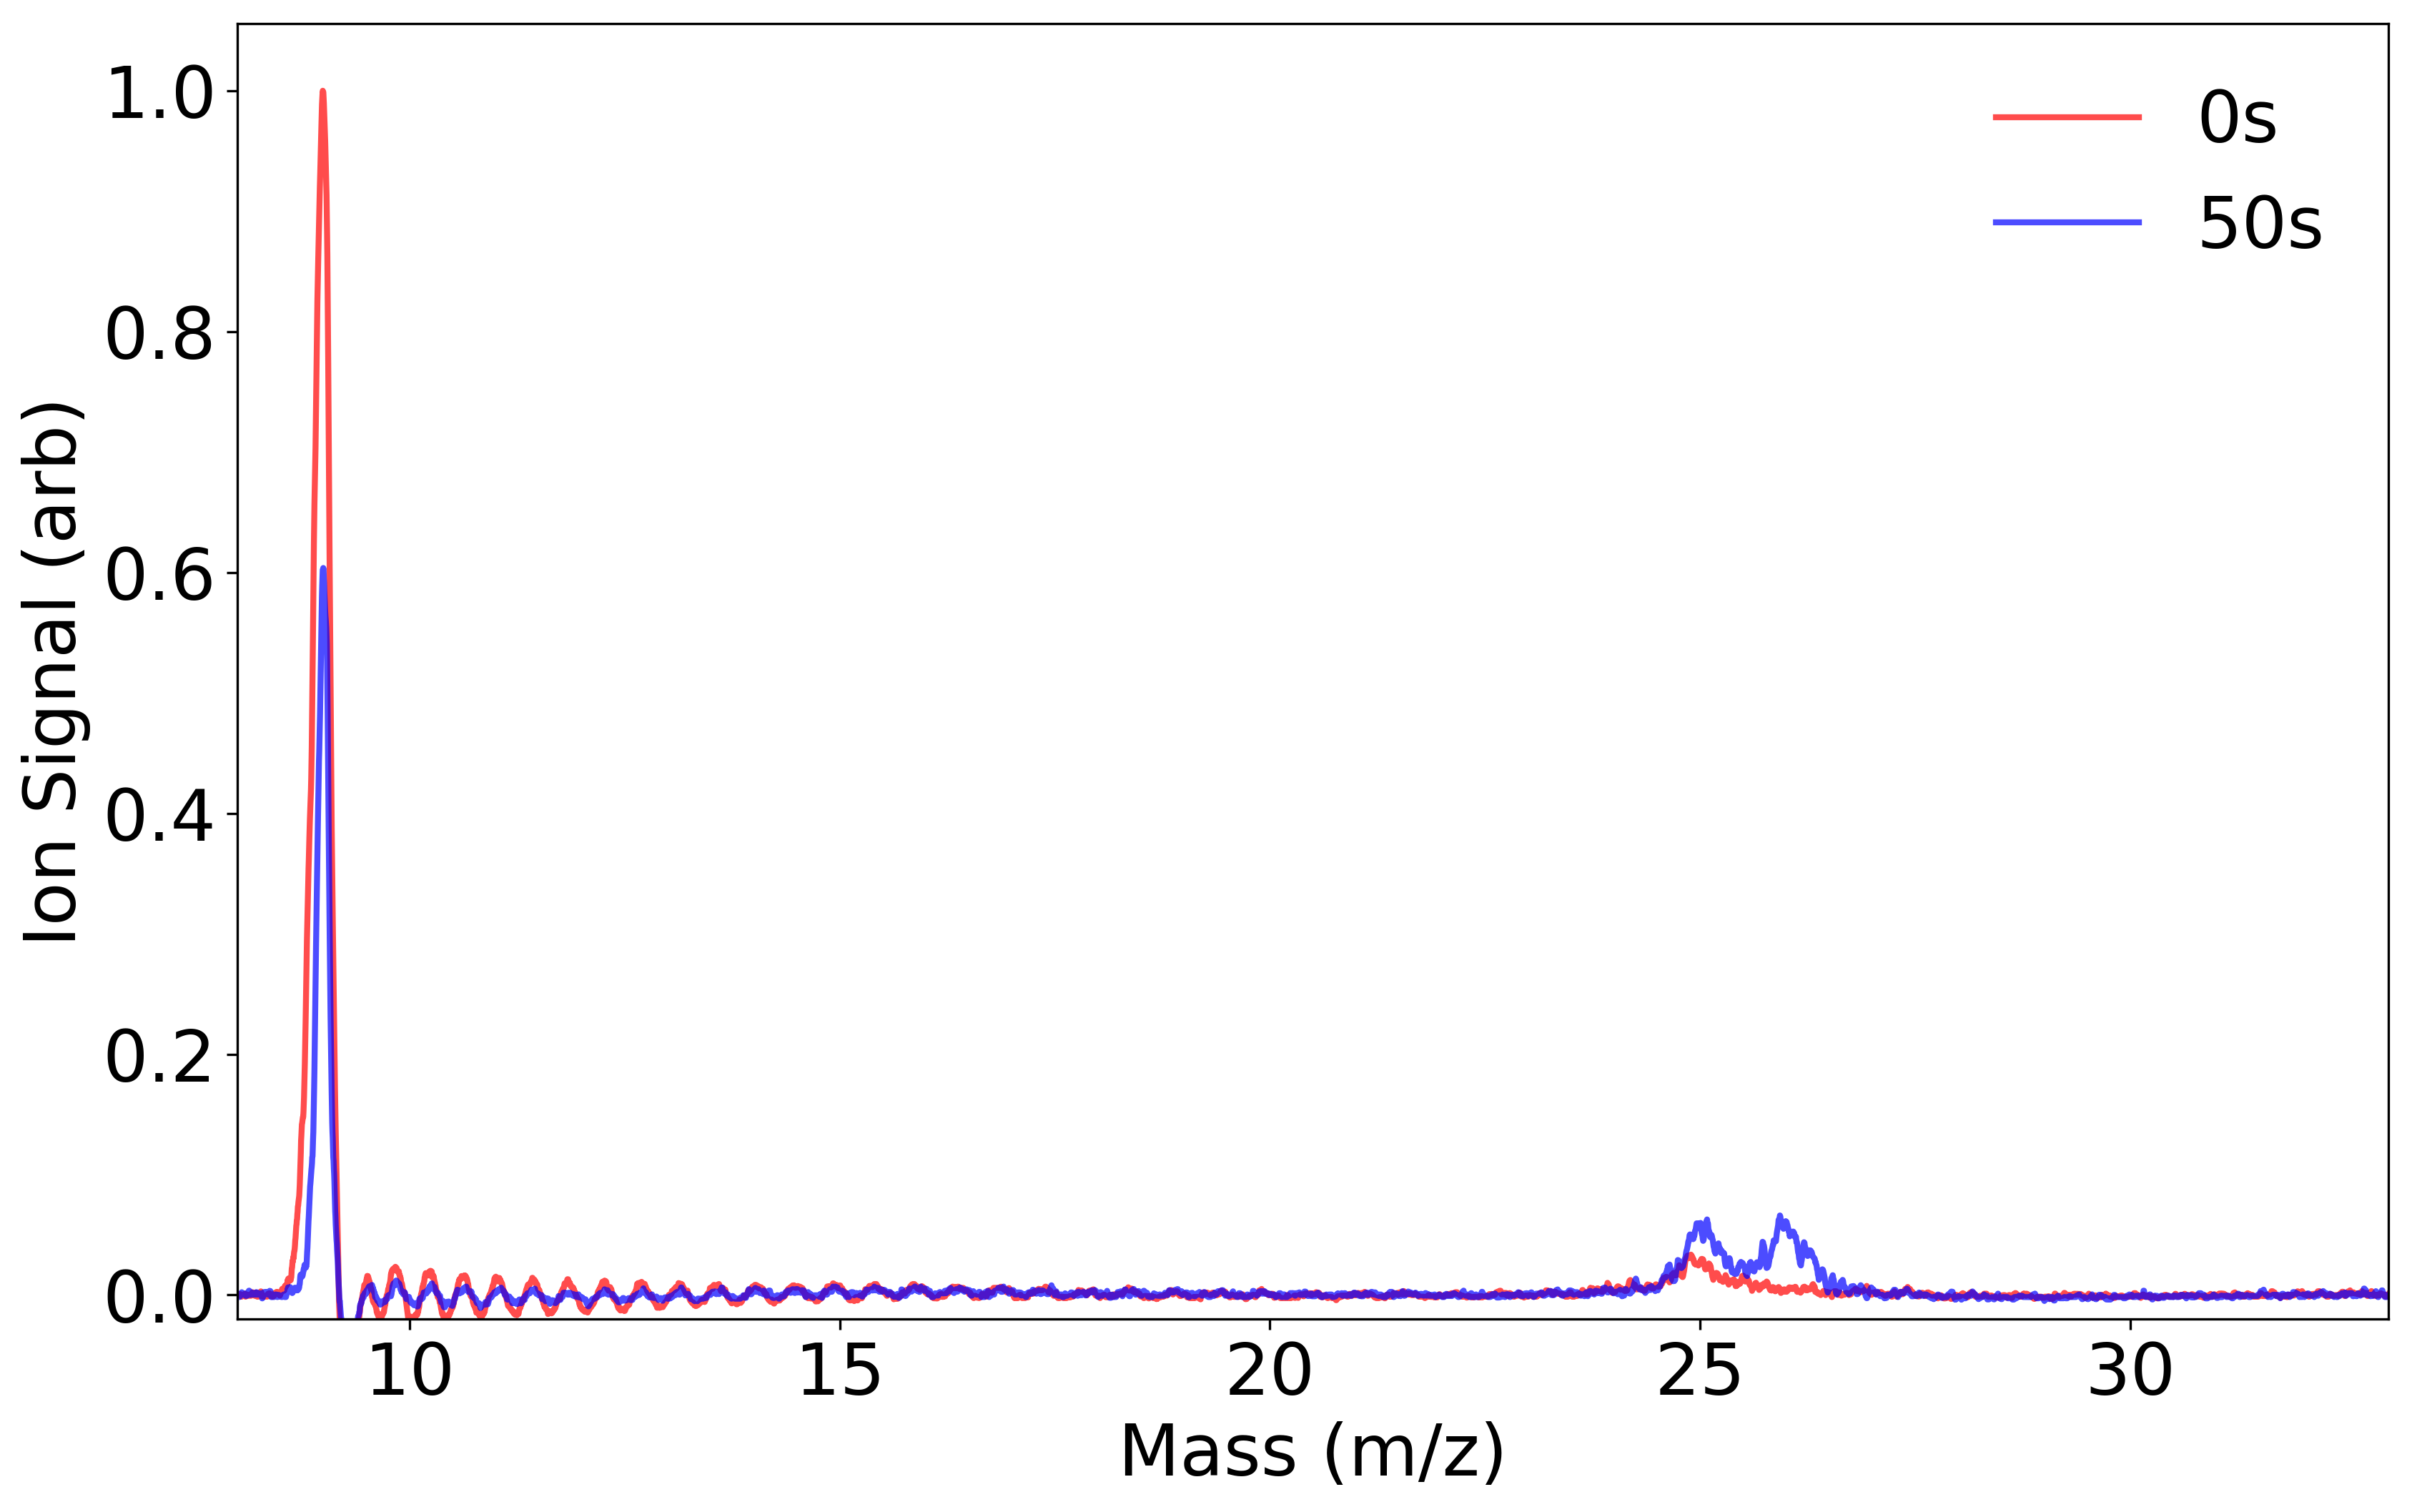
\includegraphics[width=0.7\textwidth]{images/beo_no_laser_TOF.png}
\caption{\label{fig: non laser TOF} TOF traces for data taken with 14\% p-state excitation at 0s and 200s showing no products at 0s, but distinct peaks for reaction products BeH$^+$, BeOH$^+$, and O$_2^+$.}
\end{figure}

\section{State Counting}

\begin{align}
E_{int} & = \omega_e\left(v + \frac{1}{2}\right) - \omega_ex_e\left(v+\frac{1}{2}\right)^2 + B_ej(j+1)
\end{align}

Where $\omega_e$ is the vibrational constant, $\omega_ex_e$ is the anharmonic vibrational constant, $B_e$ is the rotational constant, and $v$, $j$ are vibrational and rotational quantum numbers respectively. You can count how many states there are up to a maximum energy input and compare states to see which product channel is preferred statistically.

To get a more accurate counting, we should be comparing the integrated states including the energy taken away by the other reactant.

\begin{align}
\int_0^{p_{max}}4\pi p^2 n(p) dp
\end{align}

where $n(p)$ is the number of internal states allowed with momentum $p$


In particular, reactions \ref{eq: co} and \ref{eq: o} have been measured to have branching ratios that vary from 60:40 (CO$^+$:O$^+$) to 30:70 in the other direction. By looking at experimental data as well as the theoretical state counting, we find the ratio to be pretty definitively 60:40.